% Figura Anexo III: el juego de KYDLAND y PRESCOTT: del anuncio no creíble al equilibrio con sesgo inflacionista
\documentclass[tikz,border=3pt]{standalone}
\usepackage[T1]{fontenc}
\usepackage[utf8]{inputenc}
\usepackage{amsmath}
\usetikzlibrary{arrows.meta,calc,positioning}
\begin{document}
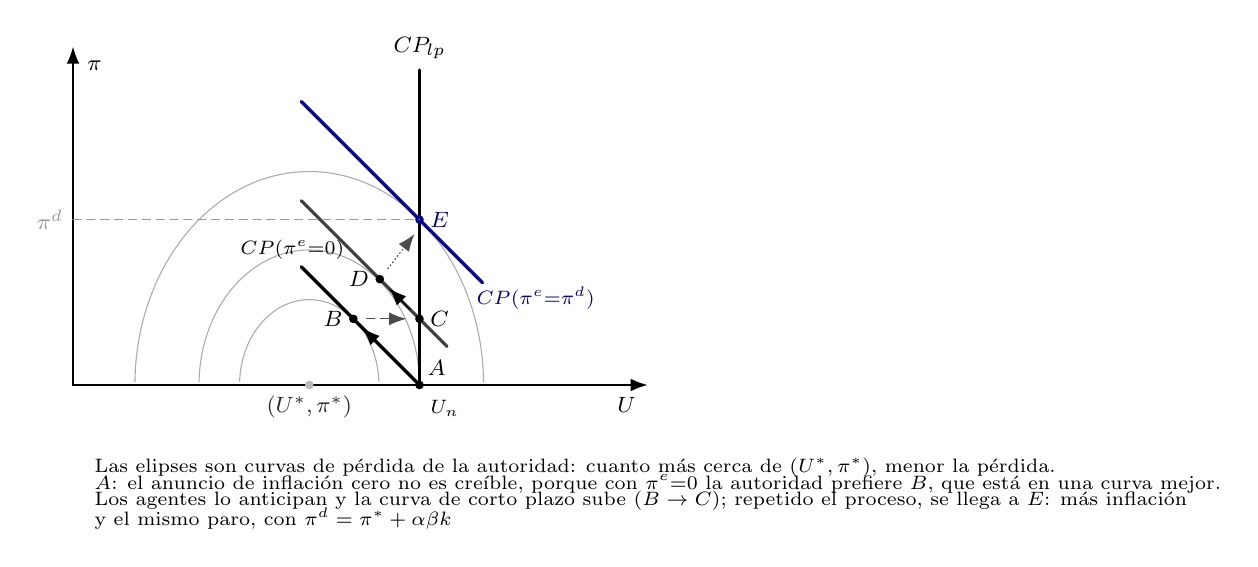
\begin{tikzpicture}[>={Latex[length=2.2mm]}, line cap=round, font=\footnotesize,
  eje/.style={->, thick},
  curva/.style={very thick},
  nueva/.style={very thick, blue!55!black},
  guia/.style={densely dashed, gray!80},
  perdida/.style={gray!65},
  pto/.style={circle, fill=black, inner sep=1.1pt}]
  \draw[eje] (0,0) -- (7.3,0) node[below left=1pt]{$U$};
  \draw[eje] (0,0) -- (0,4.3) node[below right=2pt]{$\pi$};
  % Curvas de perdida (preferencias sociales), centradas en (3, 0)
  \begin{scope}
    \clip (0.08,0.04) rectangle (7.0,4.15);
    \draw[perdida] (3,0) ellipse (0.885 and 1.084);
    \draw[perdida] (3,0) ellipse (1.4 and 1.715);
    \draw[perdida] (3,0) ellipse (2.214 and 2.711);
  \end{scope}
  \node[pto, fill=gray!55] (bliss) at (3,0) {};
  \node[below=1pt of bliss, inner sep=1pt, gray!30!black] {$(U^{*},\pi^{*})$};
  % Phillips de largo plazo
  \draw[curva] (4.4,0) -- (4.4,4.0) node[above]{$CP_{lp}$};
  % Phillips de corto plazo
  \draw[curva] (2.9,1.5) -- (4.4,0);
  \node[anchor=west, font=\scriptsize] at (2.0,1.72) {$CP(\pi^{e}{=}0)$};
  \draw[curva, gray!50!black] (2.9,2.34) -- (4.75,0.49);
  \draw[nueva] (2.9,3.6) -- (5.2,1.3);
  \node[anchor=west, font=\scriptsize, blue!55!black] at (5.0,1.1) {$CP(\pi^{e}{=}\pi^{d})$};
  % Escalera A -> B -> C -> D -> E
  \node[pto] (A) at (4.4,0) {};
  \node[inner sep=1pt] at (4.62,0.22) {$A$};
  \node[pto] (B) at (3.56,0.84) {};
  \node[left=1pt of B, inner sep=1pt] {$B$};
  \node[pto] (C) at (4.4,0.84) {};
  \node[right=1pt of C, inner sep=1pt] {$C$};
  \node[pto] (D) at (3.896,1.344) {};
  \node[left=1pt of D, inner sep=1pt] {$D$};
  \node[pto, fill=blue!55!black] (E) at (4.4,2.1) {};
  \node[right=1pt of E, inner sep=1pt, blue!55!black] {$E$};
  \draw[->, shorten >=3pt, shorten <=3pt] (A) -- (B);
  \draw[->, densely dashed, gray!60!black, shorten >=3pt, shorten <=3pt] (B) -- (C);
  \draw[->, shorten >=3pt, shorten <=3pt] (C) -- (D);
  \draw[->, densely dotted, gray!60!black, shorten >=3pt, shorten <=3pt] (D) -- (4.4,2.0);
  \draw[guia] (0,2.1) node[left]{$\pi^{d}$} -- (4.4,2.1);
  \node[below=2pt] at (4.4,0) {};
  \node[font=\scriptsize] at (4.72,-0.3) {$U_n$};
  \node[align=left, anchor=north west, font=\scriptsize] at (0.15,-0.8) {Las elipses son curvas de pérdida de la autoridad: cuanto más cerca de $(U^{*},\pi^{*})$, menor la pérdida.\\[-2pt]$A$: el anuncio de inflación cero no es creíble, porque con $\pi^{e}{=}0$ la autoridad prefiere $B$, que está en una curva mejor.\\[-2pt]Los agentes lo anticipan y la curva de corto plazo sube ($B\to C$); repetido el proceso, se llega a $E$: más inflación\\[-2pt]y el mismo paro, con $\pi^{d}=\pi^{*}+\alpha\beta k$};
\end{tikzpicture}
\end{document}
